\documentclass[a4paper,american,floatfix,pdftex,superscriptaddress,twoside,%
aps,pra,
% citeautoscript,% leave away for latexdiff
linenumbers,% remove for arXiv
% longbibliography,% not needed for revtex 4.2
% preprint,%
% galley,%
reprint,%final% add final to see real layout, no todonotes anymore, ...
]{revtex4-2}%
\usepackage{amsfonts,amsmath,amssymb}
\usepackage[T1]{fontenc}
\usepackage{graphicx}%
\usepackage[utf8]{inputenc}
\usepackage{mathtools}
\usepackage{hyperref, hypernat}
\usepackage[displaymath,textmath,graphics]{preview}

\graphicspath{{./figures/}} % define figure directory

\newcommand{\cfeldesy}{\affiliation{Center for Free-Electron Laser Science, Deutsches
      Elektronen-Synchrotron DESY, Notkestraße 85, 22607 Hamburg, Germany}}%
\newcommand{\ezemail}{\email{emil.zak@cfel.de}}%


\begin{document}
\title{CHIRALEX: theory}

\author{Emil J.\ Zak}\ezemail\cfeldesy% 
\date{\today}%
\begin{abstract}\noindent%


\end{abstract}
\maketitle%

\section{Introduction}
For gaining  direct access into the physics in the molecular frame, it is imperative to maximally confine at least one of the 
molecule's axes along a laboratory-fixed direction. Experiments utilizing  
high-harmonic generation 
(HHG)~\cite{Spector:NatComm:5:3190,Lock:PRL108:133901,Cireasa2015,piewanowski2014,Woerner:Nature466:604,Baykusheva:PRX8:031060,He2020},

 \begin{figure}
 	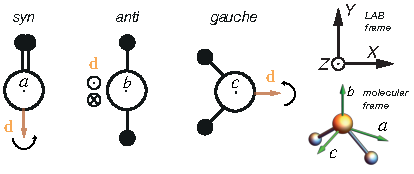
\includegraphics[width=1.0\linewidth]{Fig1}%
 	\caption{Schematic view of an asymmetric top molecule rotating about its $a$-, $b$- and $c$- principal inertia axis. From the 
 		laboratory frame perspective the molecules are in \textit{syn}, \textit{anti} and \textit{gauche} geometry. We assume that the 
 		probe pulse propagates along the laboratory $Z$-direction, whereas the molecule-confining pulse is restricted to the $XY$ 
 		plane. $d$ denotes the dipole moment vector. }
 	\label{fig:scheme}
 \end{figure}
 

\begin{widetext}
	\[
\begin{split}
\langle \cos^2 \phi \rangle_{\psi(t)}  &=  \frac{1}{16\pi^2} \sum_{J,J' =J_{min}}^{J_{max}} c_J^* c_{J'} \sqrt{(2J+1)(2J'+1)}\times 
\int_{0}^{2\pi} 
d\phi \cos^2\phi e^{-i\phi \Delta J} \sum_{K,K'=0}^{J,J'} a^{J,h_J,\tau*}_K a^{J',h_J',\tau'}_{K'}\times \\
 & \times \int d\Omega \left[
e^{-i\Delta_- K\chi}d^{J'}_{J'K'}d^{J}_{JK}+e^{i\Delta_- K\chi}d^{J'}_{J',-K'}d^{J}_{J,-K}+ 
(-1)^{\tau}(e^{i\Delta_+ K\chi}d^{J'}_{J',-K'}d^{J}_{J,K}
+e^{-i\Delta_+ K\chi}d^{J'}_{J',K'}d^{J}_{J,-K})
\right]
\end{split}
	\]
\end{widetext}
where $\Delta J = J'-J$, $\Delta_{\pm} K = K'\pm K$ and $d\Omega = \sin\theta d\theta d\chi$. Integrals over the $\phi$ angle 
impose 
rigorous selection rules on total angular momentum coupled by the $\cos ^2\phi$ operator:
\begin{equation}
\begin{split}
\int_{0}^{2\pi} 
d\phi \cos^2\phi e^{-i\phi \Delta J}  =   
\begin{cases}
2\frac{\sin(\pi \Delta J)}{\Delta J}\frac{\Delta J^2 -2}{\Delta J ^2 -4} e^{-i\pi\Delta J},& \text{if } \Delta J\neq  2\\
\frac{\pi}{2},              & \text{if} \; \Delta J = 2
\end{cases}
\end{split}
\label{eq:intphi}
\end{equation}
we note that the integral given in~\eqref{eq:intphi} is non-zero only if $\Delta J = 2$. The integral over the $\chi$ Euler angle can 
also be carried out analytically:
\begin{equation}
\begin{split}
\int_{0}^{2\pi} 
d\phi  e^{-i\phi \Delta_{\pm} K}  =   
\begin{cases}
-\frac{i}{\Delta_{\pm}K}(1-e^{-i2\pi\Delta_{\pm}K}), & \text{if }\Delta_{\pm} K\neq  0\\
2\pi,              & \text{if} \; \Delta_{\pm} K = 0
\end{cases}
\end{split}
\label{eq:intchi}
\end{equation}
whereas appropriate integrals over the azimuthal Euler angle $\theta$ are generally denoted as:
\begin{equation}
b_{JJ'KK'} = \int_0^{\pi} d\theta \sin\theta d^{J}_{J,K}(\theta) d^{J'}_{J',K'}(\theta)
\label{eq:inttheta}
\end{equation}
Equation ~\eqref{eq:intchi} restricts contributions to the alignment cosine from states with the same $K$ quantum number. After 
some algebra one finds explicit expression for the alignment cosine $\langle \cos^2 \phi \rangle_{\psi(t)} $:
\begin{widetext}
	\[
	\begin{split}
	\langle \cos^2 \phi \rangle_{\psi(t)}  &=  \frac{1}{8} \sum_{J =J_{min}}^{J_{max}-2} |c_J| |c_{J'}| \sqrt{(2J+1)(2J+5)}\times 
\left[2 b_{JJ+200}(1+(-1)^{\tau})Re( a^{J,h_J,\tau*}_0 a^{J+2,h_{J+2},\tau}_0)+\right. \\
&\left.+ \sum_{K\neq 0}^{J} Re( a^{J,h_J,\tau*}_K 
a^{J+2,h_{J+2},\tau}_K)(b_{JJ+2KK} + b_{JJ+2-K-K})
	\right] \cos(\omega_{J+2J}t + \Delta \phi^0_{J+2J})
	\end{split}
	\]
\end{widetext}
If we assume that only states with $K=J$ contribute significantly to the wavepacket, we arrive at the equation 
~\eqref{eq:cogcosine} from the main text, where we note that $Re( a^{J,h_J,\tau*}_J
a^{J+2,h_{J+2},\tau}_{J+2}) \approx 1$,  $d^J_{JJ}(\theta) = \cos^{2J}\frac{\theta}{2}$, $d^J_{J,-J}(\theta) = 
\sin^{2J}\frac{\theta}{2}$ and $b_{JJ+2JJ} =  b_{JJ+2-J-J} = \frac{2}{2J+3}$. 

\bibliography{string,cmi,b-rotation}
\end{document}

%% Local Variables:
%% coding: utf-8
%% mode: LaTeX
%% mode: auto-fill
%% mode: flyspell
%% fill-column: 100
%% ispell-dictionary: "american"
%% reftex-cite-format: default
%% TeX-auto-save: t
%% TeX-close-quote: "''"
%% TeX-open-quote: "``"
%% TeX-parse-self: t
%% truncate-lines: t
%% End:
